%!TEX root = tables.tex

\section{Conditional Diversification Benefit} % (fold)
\label{sec:conditional_diversification_benefit}

% What is CDB? Why? Non-normality, higher moments
The following description is based on~\textcite{ChristoffersenErrunzaJacobLanglois2012}, who have developed a measure of diversification in a portfolio called \emph{conditional diversification benefit} (CDB). CDB is based on the portfolio expected shortfall (ES), and therefore the full portfolio distribution.\footnote{We report results based on the distributions of our symmetric dynamic copula model.} Thus, it is able to capture higher-order moments and non-linear dependence not reflected in the covariance matrix of returns. In this context, it has the additional benefit of not being dependent on levels of expected return. ES is defined as the expected loss in some bottom percentile $q$
\begin{align}
    \text{ES}_{i,t}^q(r_{i,t}) = -\mathbb{E}[r_{i,t} | r_{i,t} \leq F_{i,t}^{-1}(q)]
\end{align}
where $F_{i,t}^{-1}(q)$ is the inverse CDF of simple returns $r_{i,t}$ at $q$ (equivalent to the $q\%$ Value-at-Risk). 

Intuitively, if assets offer little diversification, then no combination of assets will reduce total portfolio risk; and ES will be high. For a portfolio of assets with weights $w$, the portfolio's ES as a function of weights, $\text{ES}_t^q(w)$ has an upper bound equal to the weighted average of asset ES, corresponding to no diversification~\autocite{Artzner1999}:
\begin{align}
  \overline{\text{ES}}_t^q(w) = \sum_{i=1}^N w_i \text{ES}_{i,t}^q(r_{i,t})
\end{align}
A lower bound on portfolio ES corresponds to the portfolio's Value-at-Risk ($-F_{t}^{-1}(w, q)$), corresponding to perfect diversification:
\begin{align}
  \underline{\text{ES}}_t^q(w) = -F_{t}^{-1}(w, q)
\end{align}
CDB is defined as portfolio ES scaled by these bounds:
\begin{align}
  \text{CDB}_t^q(w) = \frac{\overline{\text{ES}}_t^q(w) - \text{ES}_t^q(w)}{\overline{\text{ES}}_t^q(w) - \underline{\text{ES}}_t^q(w)}
\end{align}
CDB is a number between 0 and 1 where 1 represents perfect diversification, and 0 no diversification (we present CDB scaled by 100).

Each week, we construct portfolios that maximize the 5\% CDB of portfolios with respect to portfolio weights, under the same conditions as for the mean-variance exercise (all weights sum to one; all weights positive).\footnote{Results for other levels of CDB are qualitatively similar.} Such a portfolio corresponds to the maximum degree of diversification available while being fully invested across factors. Expected shortfall is computed based on the simulated return distributions in each period, as modeled by the copula.

% Picture different between 5-factor and 6-factor
\autoref{fig:cdb} plots conditional diversification benefit measures of the six different strategies, based on the symmetric dynamic copula model. We have smoothed the plots to quarterly moving averages in order to make them easier to read. There are a number of interesting results emerging from this picture.

\begin{figure}
  \caption{5\% Conditional diversification benefit (CDB) from symmetric dynamic copula model for six different strategies, full sample (1963--2016). The line has been smoothed with a moving average on a quarterly window to make it easier to read.}
  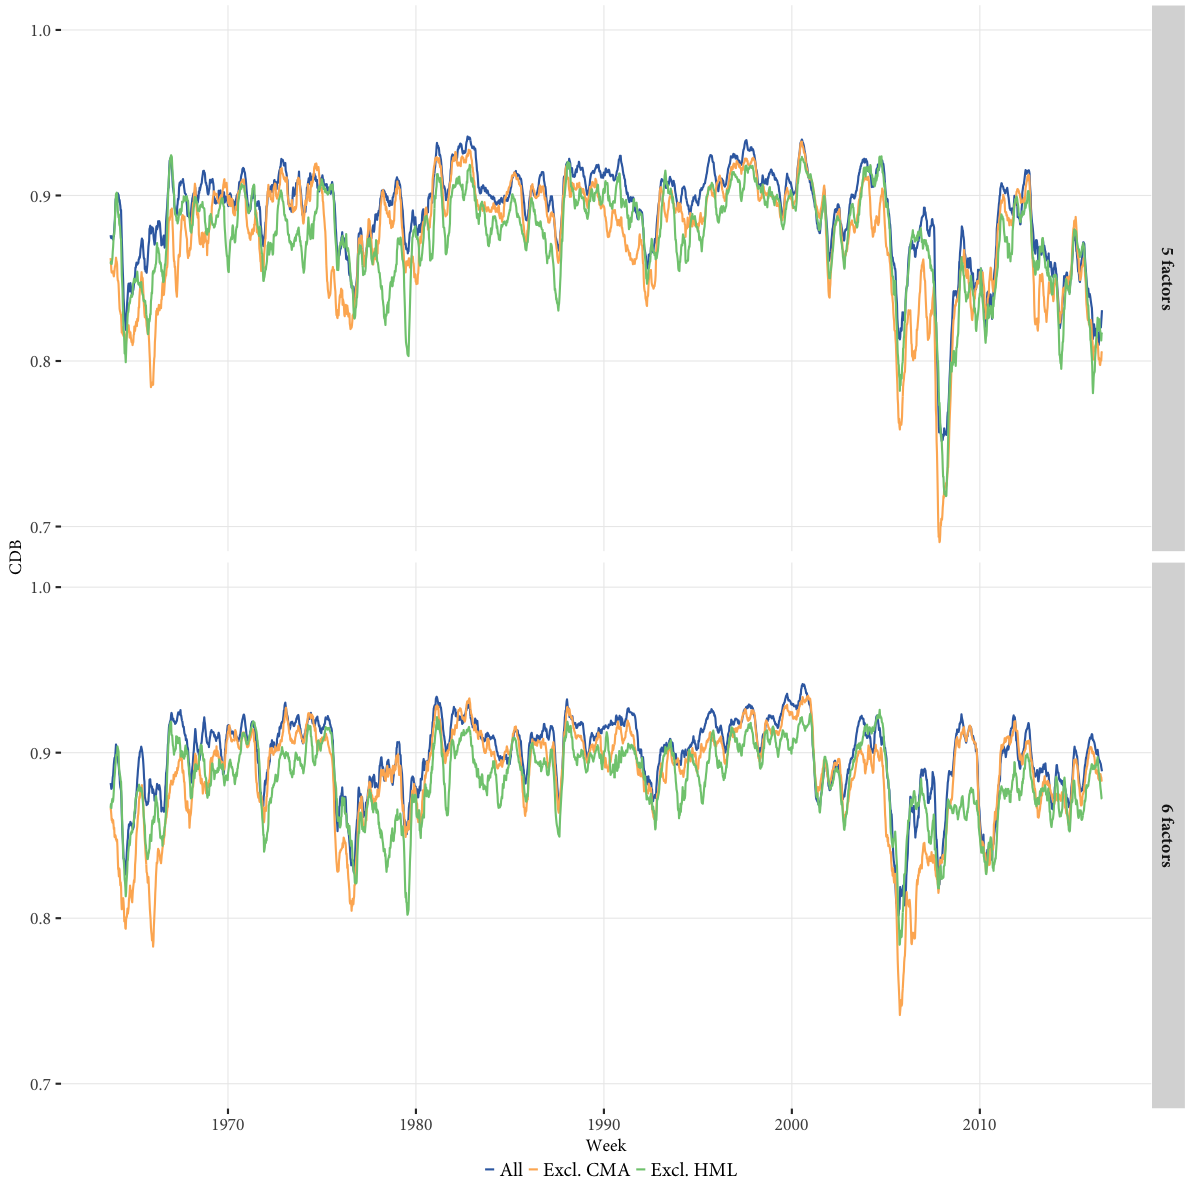
\includegraphics[width=\textwidth]{graphics/cdb_5F_6F.png}
  \label{fig:cdb}
\end{figure}

% CDB is very high; factor strategies are good diversifiers
First, we note that regardless of whether Momentum is included or not, factor strategies appear to offer high levels of diversification. In absolute terms, all strategies sit close to or above $90$ for the majority of the studied time period. The differences between strategies are small with a high degree of overlap; given the uncertainty in estimates, the interpretation of differences must be interpreted conservatively.

% Dips
Second, there are notable ``dips'' in the diversification benefit measures. When we turn to look at these dips, representing times when diversification is relatively hard to come by, we see that they roughly coincide in both the five and six factor models.

% HML is a better diversifier on average
% CMA better when diversification is hard to come by
Third, in comparing the diversification benefits offered by substituting CMA for HML and vice versa, a complicated picture appears. Looking at the six factor portfolio, the strategy where HML is excluded has a lower level of diversification benefit on most weeks compared to where CMA is excluded. This pattern appears reversed at critical times, however. When the full six factor CDB is low -- before 1965, around 1978, 2007 and 2011 -- the maximum diversification benefit of an HML strategy is in all cases except 2011 below that of the CMA strategy. HML thus appears to be the better diversifier in ``normal'' times, however, when diversification is hard to come by, CMA outperforms it. Excluding Momentum, the status of HML as a superior diversifier in normal times is much less clear; while its underperformance is even more noticeable when diversification potential is lower.

\autoref{tab:cdb_table} displays CDB summary statistics and the results of paired t-tests of the differences between strategies. This table tells the same story as the graph. In a five-factor setting, there is no significant difference in the expected diversification benefit from swapping CMA for HML, however, HML is a significantly better diversifier in a six-factor setting. The difference, although significant when taking the model as given, is however small.

%!TEX root = ../../main.tex

\begin{table}
  \centering
  \footnotesize
  \renewcommand{\arraystretch}{1.2}
  
  \caption{Conditional diversification benefit (CDB)\\ \quad \\
  Based on symmetric dynamic copula model, full sample (1963--2016). \emph{Difference} shows the average pair-wise difference in CDB between the column's and row's strategy, respectively, with t-test standard errors and significance levels (the first pair is thus the difference in pair-wise CDB between a five-factor strategy with and without CMA)}

  \begin{tabularx}{\textwidth}{@{} l X dddd X dd @{}}
    \toprule
    &&
      \multicolumn{4}{c}{CDB} && 
      \multicolumn{2}{c}{Difference} \\
    \cmidrule{3-6} \cmidrule{8-9}
    &&
      \multicolumn{1}{c}{Mean} &
      \multicolumn{1}{c}{SD} &
      \multicolumn{1}{c}{Min} &
      \multicolumn{1}{c}{Max} &&
      \multicolumn{1}{c}{All} &
      \multicolumn{1}{c}{Excl. CMA} \\
    \midrule
    \textbf{Five Factors} \\
    \emph{All}       && 88.937 & 3.410 & 61.469 & 95.135 &&   &                        \\
                     &&        &       &        &        &&   &                        \\
    \emph{excl. CMA} && 87.439 & 4.221 & 61.346 & 95.105 &&   1.497^{***} &             \\
                     &&        &       &        &        &&  (0.053)      &             \\
    \emph{excl. HML} && 87.448 & 3.731 & 61.722 & 94.274 &&   1.489^{***} & -0.009      \\
                     &&        &       &        &        &&  (0.050)      & (0.065)     \\
    \midrule
    \textbf{Six Factors} \\
    \emph{All}       && 89.783 & 2.898 & 72.850 & 95.043 &&   &                       \\
                     &&        &       &        &        &&   &                       \\
    \emph{excl. CMA} && 88.602 & 3.657 & 69.143 & 95.160 &&  1.181^{***} &             \\
                     &&        &       &        &        && (0.050)      &             \\
    \emph{excl. HML} && 88.259 & 3.053 & 71.987 & 94.447 &&  1.524^{***} &  0.343^{***}  \\
                     &&        &       &        &        && (0.049)      & (0.060)     \\
    \bottomrule
  \end{tabularx}

  \label{tab:cdb_table}
\end{table}


% What periods does low CDB correspond to?
% Story related to threshold correlations and patterns seen Mkt-HML

% No obvious corresponde with the market's performance. This does not appear
% to be related to the tail dependency so mcuh...

% subsection conditional_diversification_benefit (end)
